\chapter{Introduction}

\label{Chapter-Introduction}

Since the invention of the first computer, humankind is rapidly solving problems that are intellectually difficult for human beings but relatively easy for computers, as such problems can be described in detail with a formal list of mathematical rules. However, problems that are easy for humans, that are solved intuitively, like distinguishing the difference between a car and a person, or a spoken word and a bird's chirp, is a real challenge for computers and engineers \cite{Goodfellow-et-al-2016}. Those problems cannot be described, at the time of writing, with sharply defined mathematical rules. Artificial Intelligence (AI) and Machine Learning (ML) study those types of problems, with many successes in the cost of highly computationally complex algorithms.

It is estimated that by the year 2025, the total amount of data created worldwide will rise to 163 ZettaBytes, while every minute of the year 2019, Americans used more than 4.4 PetaBytes of data \cite{Forbes-How-Much-Data-Is-Collected-Every-Minute-Of-The-Day}. It is evident that data management systems and knowledge extraction from them, also called Data Analysis, are urgent. Although such problems can be tackled using Artificial Intelligence and Machine Learning, it is extremely computationally intensive, if not even non-feasible, in a reasonable amount of time.

Fortunately, most of the algorithms used to tackle such problems come with high parallelism. Therefore, they can be expanded in the space domain, in other words, they can utilize more hardware resources to cut down on needs from the time domain. Of course, there are many different types of hardware resources, each with their advantages and disadvantages, from parallelism capabilities and energy efficiency to cost of production, reconfigurability, and reusability.

\section{Motivation}
Nowadays, the computational complexity of the aforementioned algorithms makes hardware acceleration a necessity, since running them on Central Processing Units (CPUs) is, while possible, the least efficient and fast solution. Although writing software for CPUs may be fast and easy, its running speed due to low parallelism and high power consumption, as a general propose piece of hardware, are far from ideal. For reference, at the time of writing, a top-grade server CPU, AMD EPYC 7002 Series (Figure \ref{fig:amd-epyc-7002-chip}), can provide up to 64 cores and 128 threads, at up to 2.25GHz base clock and 3.4GHz boost clock, with a rated Thermal Design Power (TDP) of 225Watts, and a list price of 4,425 USD \cite{AMD-EPYC-7002-Series-Processors}.

\begin{figure} [H]
	\centering
	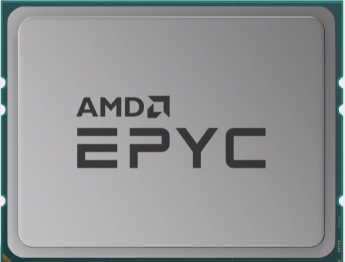
\includegraphics[scale=0.45]{Images/Hardware/amd-epyc.png}
	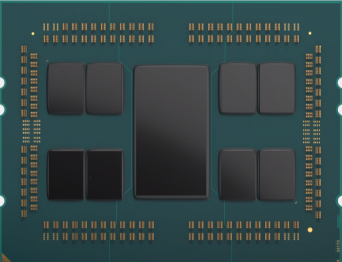
\includegraphics[scale=0.45]{Images/Hardware/amd-epyc-dies.png}
	\decoRule
	\caption[AMD Epyc 7002 series chip]{AMD Epyc 7002 series chip: \href{https://www.amd.com/en/processors/epyc-7002-series}{URL}}
	\label{fig:amd-epyc-7002-chip}
\end{figure}

Graphics Processing Units (GPUs), on the other hand, provide much higher parallelism, while still being relatively easy for their software to be written. However, they can be costly to scale up, and their power consumption can be really high. For reference, at the time of writing, a top-grade GPU for ML, NVIDIA Titan RTX (Figure \ref{fig:nvidia-titan-rtx-explosion-view}), provides up to 72 Streaming Multiprocessors, up to 4,608 CUDA Cores and up to 576 Tensor cores, with a rated base clock of 1,350 MHz and boost clock of 1,770 MHz, 24 GB of Graphics Double Data Rate (GDDR6) Memory and a power consumption of 280 Watts for 2,500 USD \cite{NVIDIA-Titan-RTX-GPU}.

\begin{figure} [H]
	\centering
	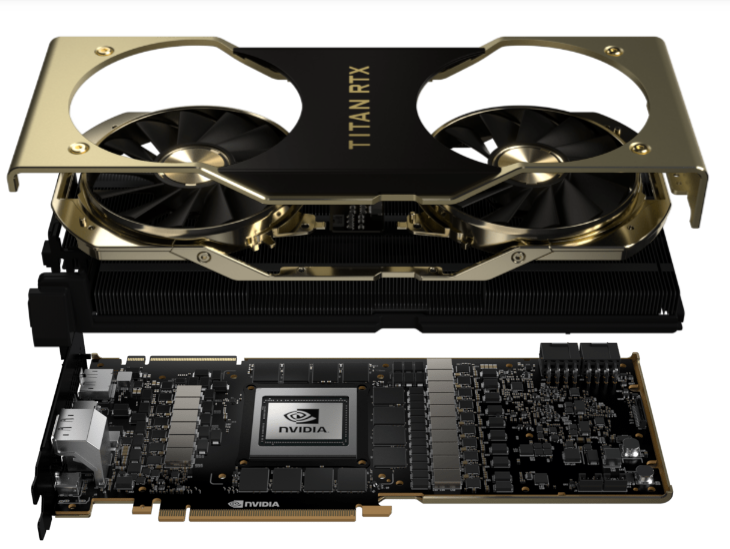
\includegraphics[scale=0.5]{Images/Hardware/NVIDIA-Titan-RTX.png}
	% 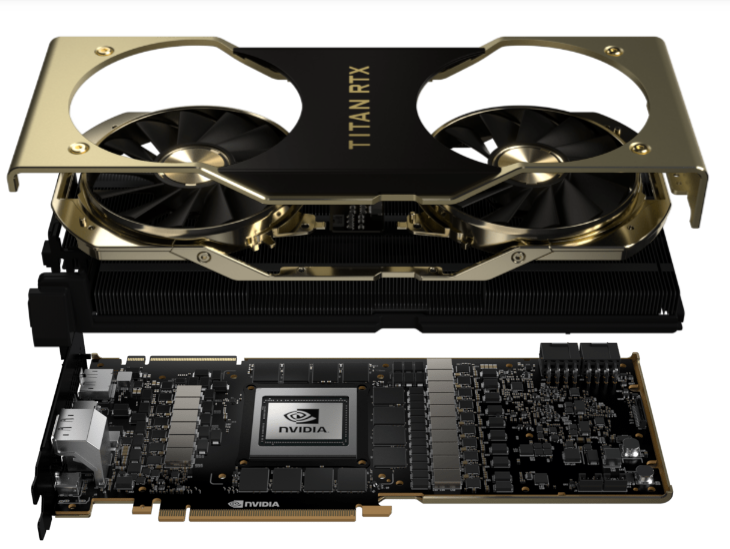
\includegraphics[width=\textwidth]{Images/Hardware/NVIDIA-Titan-RTX.png}
	\decoRule
	\caption[NVIDIA Titan RTX card]{NVIDIA Titan RTX card: \href{https://www.nvidia.com/en-us/deep-learning-ai/products/titan-rtx/}{URL}}
	\label{fig:nvidia-titan-rtx-explosion-view}
\end{figure}

Moreover, there are Application Specific Integrated Circuits (ASICs), which can provide the best parallelism capabilities and the lowest power consumption for a particular application. Unfortunately, they are very expensive to develop and produce, and they can only serve a single purpose, a single application. An example of such an ASIC is the Google Cloud Tensor Processing Unit (TPU) (Figure \ref{fig:google-tpu-motherboard}), which, for the third version (v3), in a single chip there are two TPU cores, each of which contains two scalar, vector, and matrix units (MXUs), and 16 GB of High Bandwidth Memory (HBM) \cite{Google-Cloud-TPU}.

\begin{figure} [H]
	\centering
	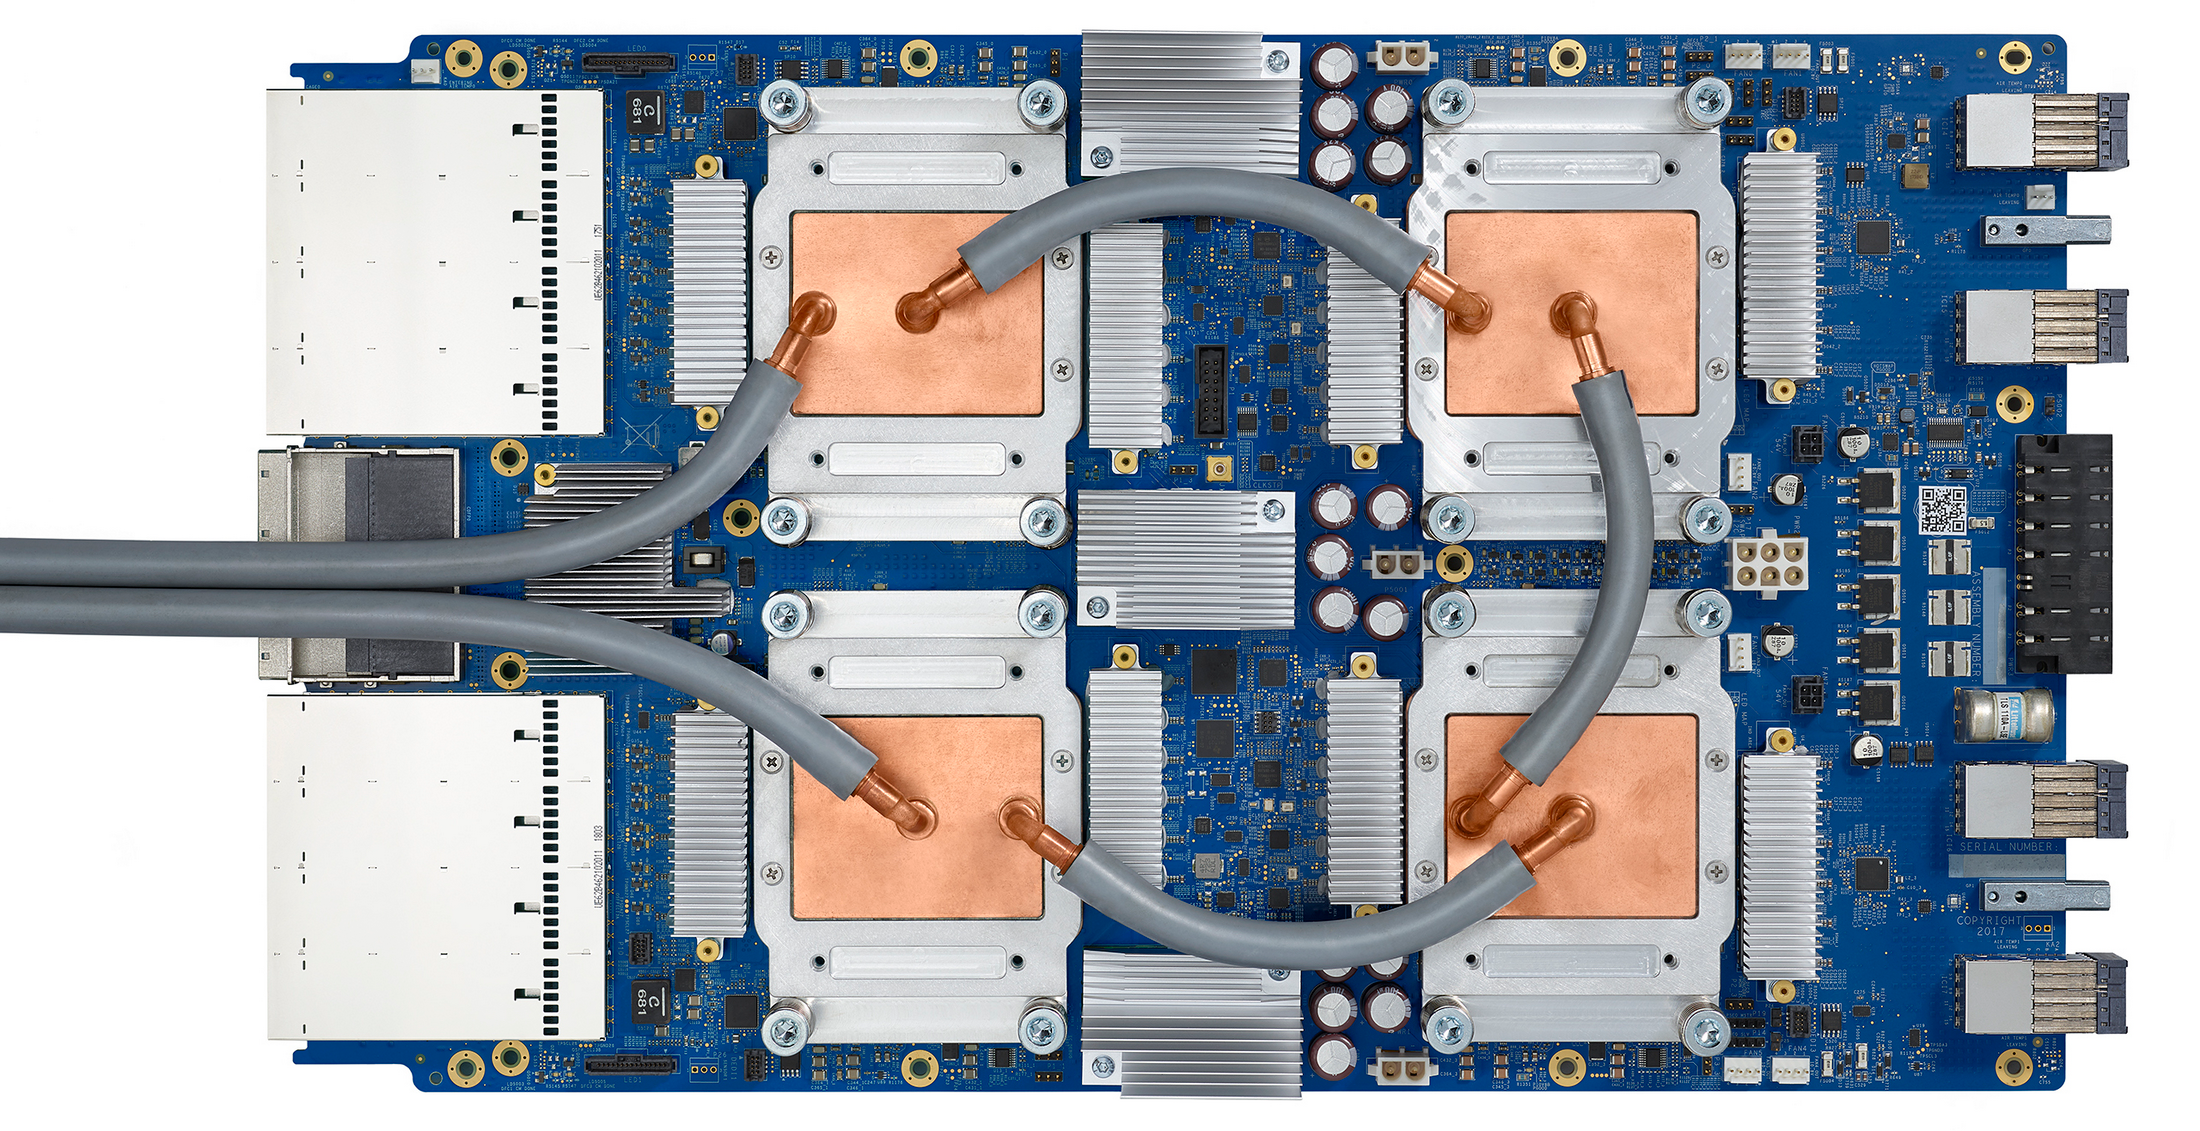
\includegraphics[width=\textwidth]{Images/Hardware/tpu-v3.png}
	\decoRule
	\caption[Google's TPU v3]{Google's TPU v3 - 4 chips, 2 cores per chip: \href{https://cloud.google.com/tpu/docs/system-architecture}{URL}}
	\label{fig:google-tpu-motherboard}
\end{figure}

On the contrary, Field Programmable Gate Arrays (FPGAs) are bridging the gap between the GPUs' flexibility and the ASICs' performance and power consumption. An example FPGA Hardware targeted for High-Performance Computing (HPC) is the Quad-FPGA Daughter Board (QFDB) (Figure \ref{fig:forth-qfdb-daughterboard}) \cite{Implementation-and-Impact-of-an-Ultra-Compact-Multi-FPGA-Board-for-Large-System-Prototyping}, developed by the Foundation of Research and Technology Hellas (FORTH) \cite{FORTH}, combines four interconnected Xilinx Zynq Ultrascale+ Multi-Processor Systems on Chip (MPSoCs), with 16GB of DDR4 memory and an M.2 Solid State Drive (SSD).

\begin{figure} [H]
	\centering
	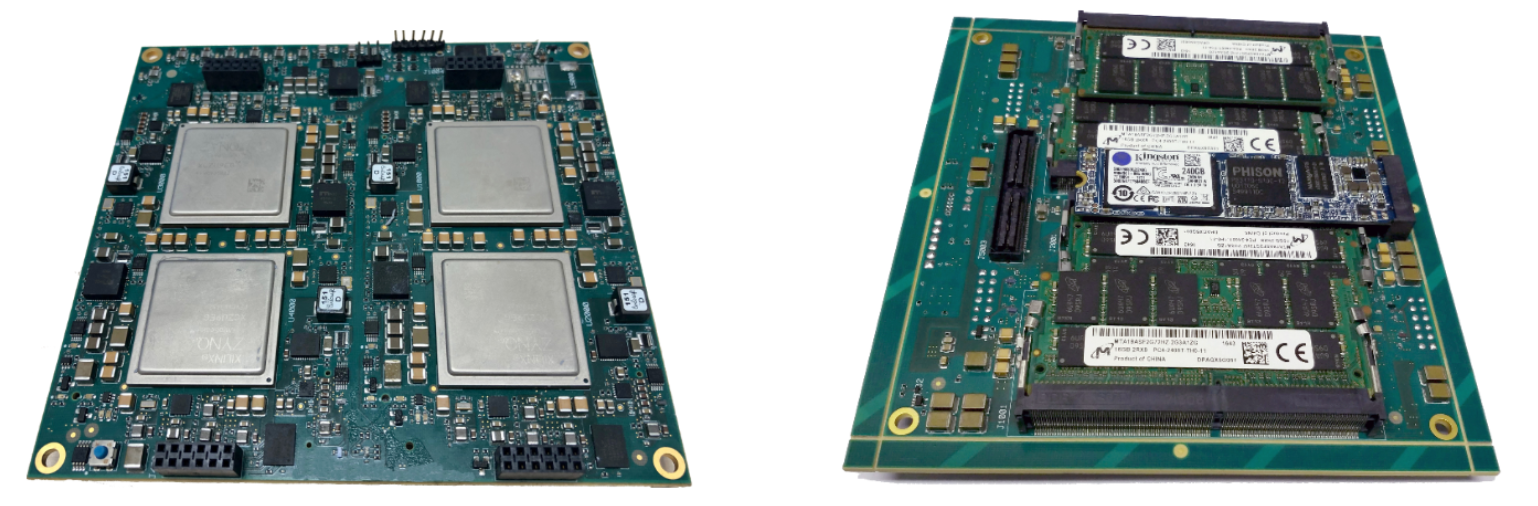
\includegraphics[scale=0.22]{Images/Hardware/QFDB.png}
	% 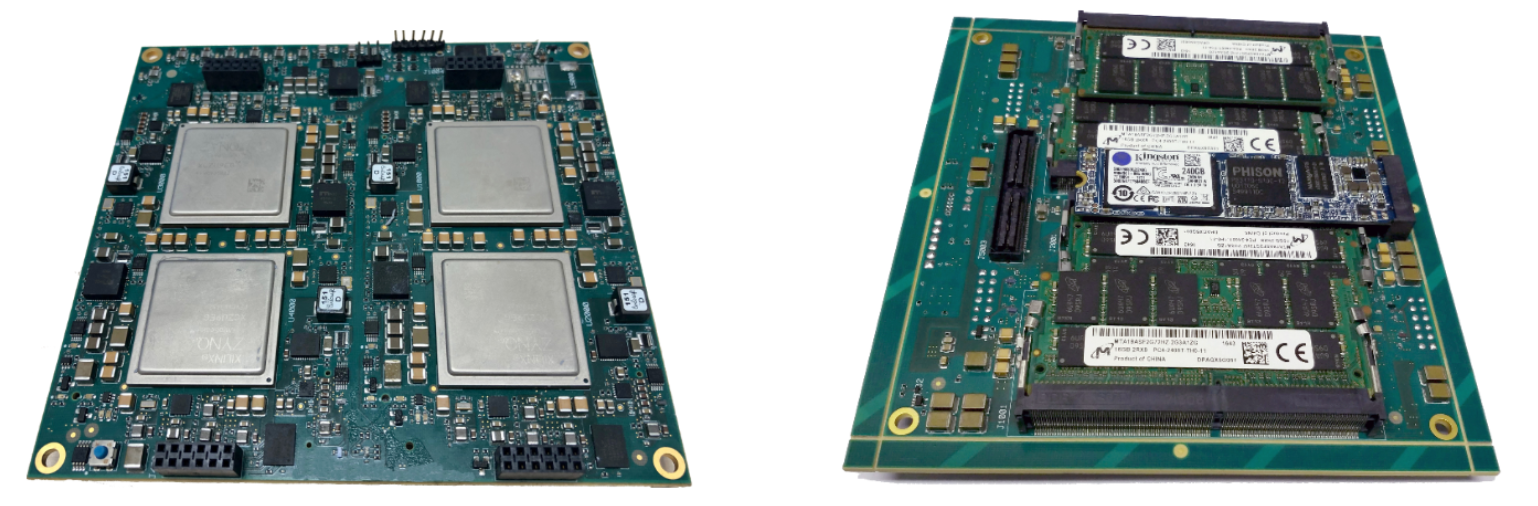
\includegraphics[width=\textwidth]{Images/Hardware/QFDB.png}\\[0.5cm]
	\decoRule
	\caption[FORTH QFDB]{FORTH QFDB, top-view (left) and bottom-view (right): \href{https://ieeexplore.ieee.org/stamp/stamp.jsp?arnumber=8945720}{URL}}
	\label{fig:forth-qfdb-daughterboard}
\end{figure}

In this work, the FPGAs' benefits are being utilized to create a hardware accelerator that can speed up the inference of Convolutional Neural Networks (CNNs), a branch of Deep Neural Networks (DNNs), which is a subfield of Machine Learning.

\section{Scientific Contributions}

\section{Thesis Outline}
\begin{itemize}
	\item \textbf{Chapter 2 - Theoretical Background:} The theoretical background of Machine Learning, with emphasis on Convolutional Neural Networks, is being described.
	\item \textbf{Chapter 3 - Related Work:} The related work on the field of Convolutional Neural Networks and their hardware implementations is being described.
	\item \textbf{Chapter 4:} Chapter 4 description
	\item \textbf{Chapter 5:} Chapter 5 description
	\item \textbf{Chapter 6:} Chapter 6 description
	\item \textbf{Chapter 7:} Chapter 7 description
\end{itemize}
